\chapter{Análisis y diseño}

%\section{Alcance del proyecto}
%uwu
%\subsection{Limitaciones y Consideraciones}

%\subsection{¿Que puede pedir el usuario?}
%uwu

\section{Casos de Uso}
En esta sección se describen los casos de uso del sistema propuesto, los cuales representan las principales interacciones entre el usuario y la solución de navegación asistida desarrollada. Los casos de uso permiten identificar las funcionalidades clave del sistema desde una perspectiva externa, enfocándose en las acciones que el usuario puede realizar y las respuestas que el sistema proporciona.

El sistema está diseñado para asistir a personas con discapacidad visual durante su desplazamiento en entornos urbanos o interiores, mediante la generación de instrucciones auditivas, la detección de obstáculos y la adaptación dinámica de rutas. En este contexto, los casos de uso modelan el flujo de interacción necesario para lograr una navegación segura y eficiente.

Los actores principales identificados son el \textbf{usuario}, quien interactúa mediante comandos de voz, y el \textbf{sistema}, el cual procesa la información del entorno y genera las respuestas correspondientes. A partir de esta interacción, se definen los distintos escenarios funcionales que permiten cumplir con los objetivos del sistema.
Los casos de uso considerados son los siguientes:
\subsubsection{Activar el sistema} 
Este caso de uso permite iniciar el funcionamiento del sistema de navegación mediante la activación del dispositivo.
El usuario presiona el botón de activación, el sistema se inicia, se activan los sensores, cámara y el modulo de reconocimiento de voz, el sistema queda listo para recibir instrucciones y el resultado esperado es que el sistema queda preparado para comenzar la navegación.
\subsubsection{Detener la navegación}
Permite finalizar el proceso de navegación y detener las instrucciones auditivas emitidas por el sistema.
El usuario solicita detener la navegación, el sistema cancela la ruta activa
y la navegación finaliza correctamente.
\subsubsection {Indicar destino}
El usuario proporciona al sistema el lugar al que desea dirigirse.
El usuario menciona el destino mediante comandos de voz, el sistema procesa la información recibida, identifica el destino solicitado, el sistema procede a la confirmación del destino. Así, el sistema obtiene correctamente el destino deseado.
\subsubsection {Confirmar destino}
El sistema valida que el destino interpretado sea correcto antes de iniciar la navegación.
El sistema comunica el destino detectado, el usuario confirma la información,
si la información es correcta, empieza la navegación.
\subsubsection {Emitir instrucciones de navegación}
El sistema proporciona instrucciones auditivas durante el recorrido hacia el destino seleccionado.
El sistema calcula la ruta, se generan instrucciones de navegación y el usuario recibe indicaciones auditivas. El resultado esperado es que el usuario recibe orientación continua durante el trayecto.
\subsubsection {Detectar y alertar obstáculos}
El sistema detecta obstáculos durante el desplazamiento y emite alertas preventivas al usuario.
Los sensores y cámaras monitorean el entorno, el sistema identifica posibles obstáculos, se genera una alerta auditiva y el resultado esperado es que el usuario evite colisiones.
\subsubsection {Recalcular ruta}
Permite recalcular una nueva ruta cuando el camino original presenta inconvenientes.
El sistema detecta un problema en la ruta actual, se calcula una ruta alternativa o se espera el guardado de una ruta nueva y el resultado es la navegación continúa mediante una ruta alternativa segura.
\subsubsection {Confirmar nueva ruta}
El usuario valida si desea continuar mediante la nueva ruta propuesta por el sistema.
El sistema informa la existencia de una nueva ruta, el usuario acepta o rechaza la alternativa; si acepta, el sistema actualiza la navegación, el resultado es la ruta alternativa confirmada y guardada.
\subsubsection {Finalizar navegación}
El sistema informa al usuario que ha llegado correctamente al destino seleccionado.
El sistema detecta la llegada al destino, se emite una notificación auditiva y finaliza el proceso de navegación.
% SE PUEDE ESCRIBIR UN POCO DE CADA USO O SE PUEDE HACER DESPUES DE PRESENTAR EL DIAGRAMA @Thaia

\subsection{Diagrama de casos de uso}

El diagrama de casos de uso mostrado en la Figura~\ref{fig:casos_uso} representa de manera gráfica las interacciones entre el usuario y el sistema, así como la relación entre los distintos casos de uso identificados.

\begin{figure}[H]
    \centering
    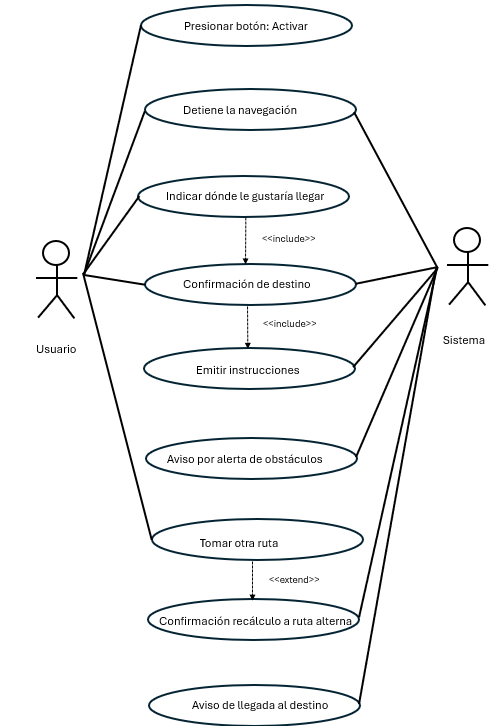
\includegraphics[width=13cm]{Diagramas/DiagCasoUso.png}
    \caption{Diagrama de casos de uso del sistema de navegación asistida}
    \label{fig:casos_uso}
\end{figure}

Este modelo permite identificar de forma clara las funcionalidades del sistema, así como las dependencias y comportamientos alternativos que pueden surgir durante su operación.
\\
El actor principal es el Usuario, quien interactúa directamente con el sistema mediante distintas funcionalidades. Por su parte, el Sistema actúa como el ente que procesa la información, toma decisiones y proporciona retroalimentación.

El usuario tiene la capacidad de activar el sistema “Presionar botón: Activar”. Este caso de uso representa la acción inicial que habilita la interacción con el sistema. Asimismo, el usuario puede detener la navegación en cualquier momento a través del caso de uso “Detiene la navegación”, lo que evidencia que el sistema debe permitir el control total sobre su ejecución.

“Indicar dónde le gustaría llegar”, donde el usuario proporciona el destino deseado. Este caso de uso describe una interacción directa en la que el sistema debe ser capaz de recibir y procesar la entrada del usuario. Asociado a este, se encuentra el caso de uso “Confirmación de destino”, el cual corresponde a una responsabilidad del sistema: validar y confirmar la información recibida. La relación <<include>> entre ambos indica que la confirmación es un comportamiento obligatorio que forma parte del servicio principal de captura de destino.

Una vez que el destino ha sido definido, el sistema ofrece la funcionalidad de “Emitir instrucciones”, que consiste en proporcionar indicaciones al usuario para llegar a su destino. Este caso de uso también está relacionado mediante <<include>>, lo que indica que depende de la confirmación previa del destino para ejecutarse correctamente.

Durante la interacción, el sistema incluye la capacidad de “Aviso por alerta de obstáculos”, lo cual representa una funcionalidad autónoma del sistema orientada a la seguridad del usuario. En este caso, el usuario no necesariamente inicia la acción, sino que el sistema actúa de manera proactiva notificando eventos relevantes del entorno.

“Tomar otra ruta”, está asociado a una relación <<extend>> con “Confirmación recálculo a ruta alterna”. Esta relación indica que se trata de una funcionalidad opcional que solo se activa bajo ciertas condiciones, como la detección de obstáculos o cambios en el entorno. En este contexto, el sistema asume la responsabilidad de recalcular una nueva ruta, mientras que el usuario participa de forma indirecta al recibir la confirmación de dicho ajuste.

El caso de uso “Aviso de llegada al destino”, representa la notificación al usuario de que se ha cumplido el objetivo de la navegación. Este caso de uso corresponde completamente al sistema, quien debe identificar el cumplimiento de la meta y comunicarlo oportunamente.

\section{Diagramas de flujo}
Con el objetivo de representar de manera detallada la secuencia operativa interna de este sistema, se emplea un diagrama de flujo, el cual describe los procesos, decisiones y ciclos que se ejecutan desde la activación del sistema hasta la llegada al destino.

\begin{figure}[H]
    \centering
    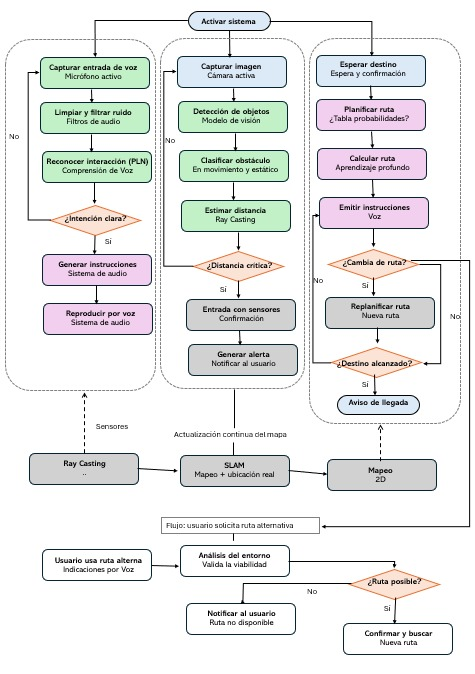
\includegraphics[width=13cm]{DiagFlujo/FlujoGeneral.jpeg}
    \caption{Diagrama de flujo global del sistema}
    \label{fig:flujo_gen}
\end{figure}
\textbf{Módulo 1 - Voz}
El sistema comienza capturando la entrada del usuario mediante el bloque “Capturar entrada de voz”, donde se utiliza el micrófono para recibir comandos. Posteriormente, la señal pasa por el proceso de “Limpiar y filtrar ruido”, en el cual se aplican técnicas de procesamiento de audio para mejorar la calidad de la señal.
\\
Una vez depurada, la información es interpretada en “Reconocer interacción (PLN)”, donde se emplean modelos de procesamiento de lenguaje natural para comprender la intención del usuario.
\\
Se presenta una decisión clave: “¿Intención clara?”.
\\
Si la respuesta es afirmativa, el sistema procede a “Generar instrucciones” y posteriormente a “Reproducir por voz”, proporcionando retroalimentación auditiva al usuario.
En caso contrario, el sistema puede requerir nueva entrada o repetir el proceso de interpretación.
\\
Este módulo es fundamental, ya que permite una interacción natural y accesible entre el usuario y el sistema.

\textbf{Módulo 2 - Visión}
\\
De manera paralela, el sistema activa la cámara en el bloque “Capturar imagen”, obteniendo información visual del entorno. Esta información es procesada en “Detección de objetos”, donde un modelo de visión identifica elementos relevantes.
\\
Posteriormente, en “Clasificar obstáculo”, el sistema determina si los objetos detectados representan un riesgo, diferenciando entre obstáculos móviles y estáticos.
\\
El siguiente paso es “Estimar distancia”, donde se calcula la proximidad de los objetos mediante técnicas como Ray Casting.
\\
Esto conduce a la decisión “¿Distancia crítica?”:
\\
Si se detecta un riesgo cercano, el sistema ejecuta “Entrada con sensores” para validar la información y posteriormente “Generar alerta”, notificando al usuario.
Si no existe riesgo, el sistema continúa monitoreando el entorno sin interrumpir la navegación.
\\
Este módulo garantiza la seguridad del usuario mediante análisis en tiempo real del entorno.

\textbf{Módulo 3 - Ruta}
En este módulo, el sistema puede encontrarse inicialmente en el estado “Esperar destino”, hasta recibir la confirmación del usuario. Una vez definido, se ejecuta “Planificar ruta”, donde se evalúan posibles trayectorias.
\\
Posteriormente, en “Calcular ruta”, se emplean algoritmos de aprendizaje profundo para determinar la mejor opción disponible. El resultado se comunica mediante “Emitir instrucciones”, guiando al usuario durante su desplazamiento.
\\
Durante la navegación, el sistema evalúa continuamente la condición “¿Cambia de ruta?”:
\\
Si no hay cambios, el sistema sigue emitiendo instrucciones.
Si ocurre un evento (por ejemplo, un obstáculo), se activa “Replanificar ruta”, generando una nueva trayectoria.
\\
Finalmente, se evalúa “¿Destino alcanzado?”:
\\
Si la respuesta es afirmativa, el sistema ejecuta “Aviso de llegada”, concluyendo el proceso.
En caso contrario, el ciclo de navegación continúa.

\textbf{Sensores y mapeo}
Se presenta:
SLAM (Mapeo y ubicación en tiempo real)
Mapeo 2D
Ray Casting
\\
Estos elementos permiten la actualización continua del entorno, proporcionando información clave a los módulos de visión y planificación. Gracias a este sistema, el modelo puede tomar decisiones informadas en tiempo real.
\\
Se contempla un flujo adicional cuando el usuario decide cambiar la ruta. Este proceso inicia en “Usuario usa ruta alterna”, seguido de un “Análisis del entorno” para validar la viabilidad.
\\
Se evalúa la decisión “¿Ruta posible?”:
\\
Si la ruta es viable, el sistema procede a “Confirmar y buscar nueva ruta”.
En caso contrario, se ejecuta “Notificar al usuario ruta no disponible”, informando la imposibilidad del cambio.
\subsection{Flujo de percepción}
Para los modulos que ayudan al sistema a percibir el mundo como el de Visión y el de los sensores, el flujo es:
El proceso interno del sistema para la detección, análisis y validación de obstáculos, integrando información proveniente de visión por computadora y sensores físicos. Su objetivo principal es garantizar que las decisiones de navegación se basen en información confiable, reduciendo falsos positivos y aumentando la seguridad del usuario.
\begin{figure}[H]
    \centering
    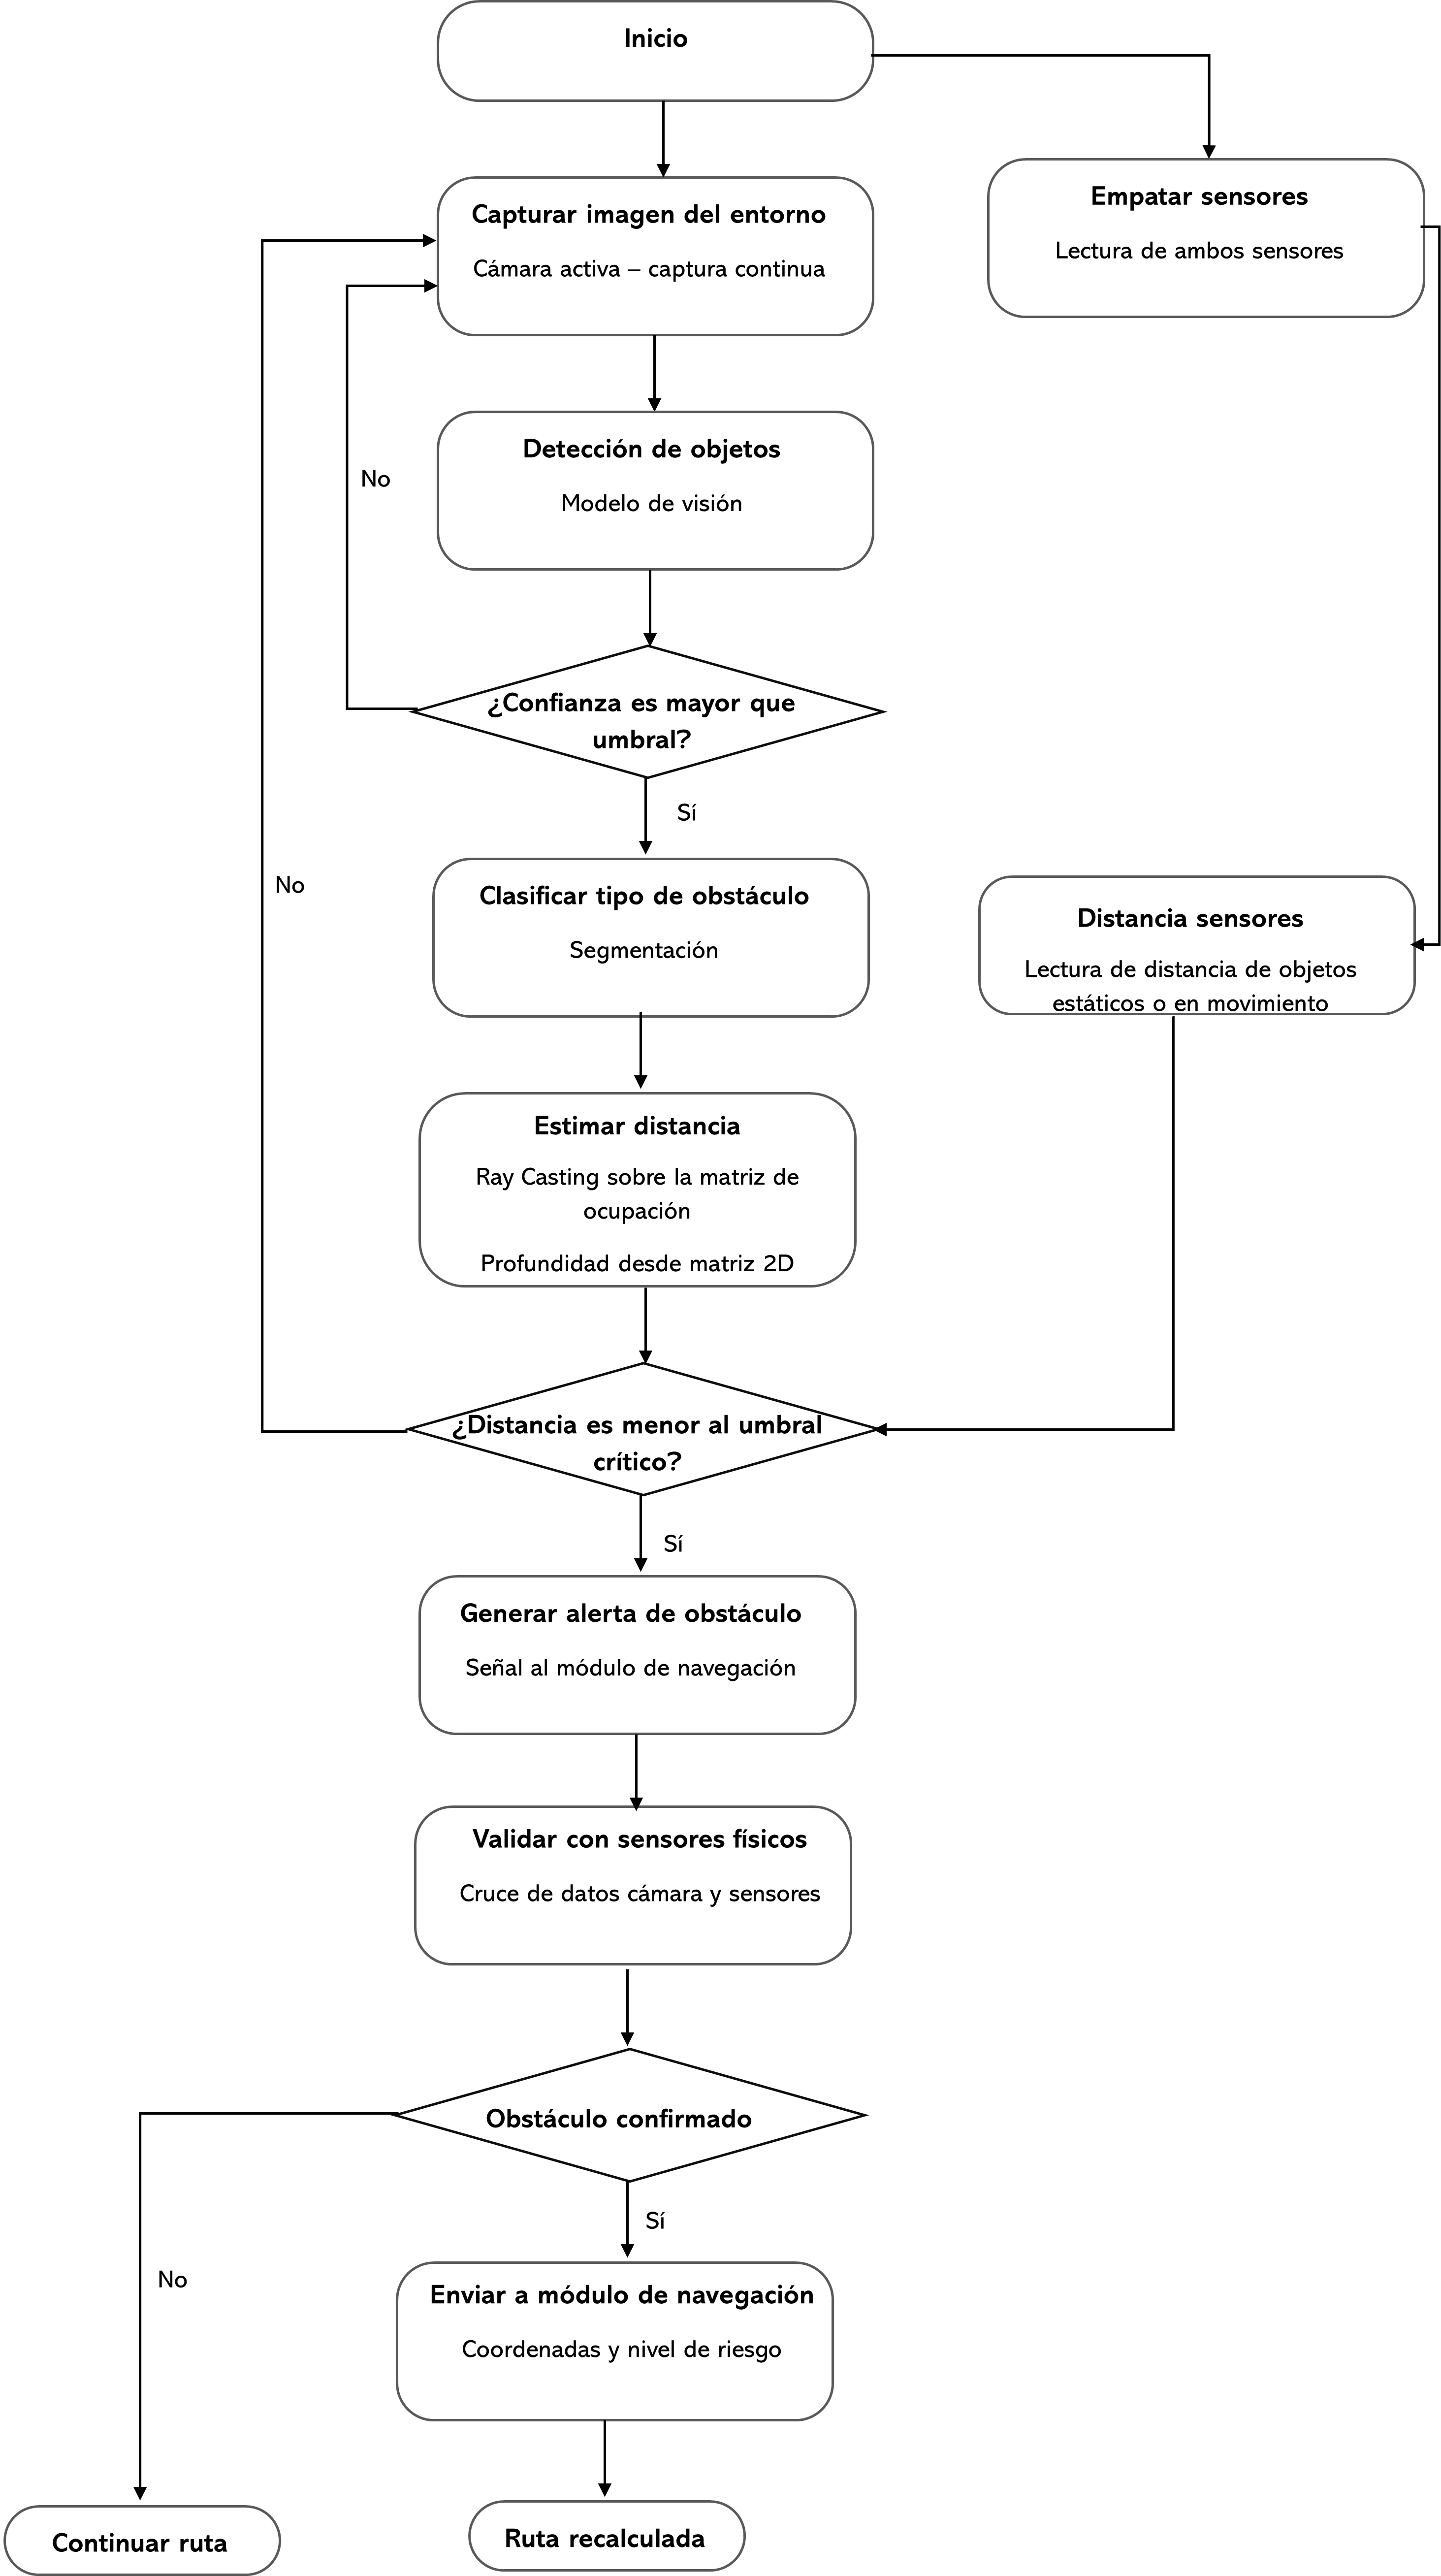
\includegraphics[width=11cm]{DiagFlujo/FlujoVision.png}
    \caption{Diagrama de flujo del Modulo de Vision y Modulo sensorial}
    \label{fig:flujo_vision}
\end{figure}
El flujo inicia a partir de dos procesos fundamentales:
Captura de imagen mediante una cámara activa y la entrada de los sensores, donde se realiza la lectura simultánea de los sensores físicos para sincronizar la información.

Una vez capturada la imagen, el sistema ejecuta el proceso de “Detección de objetos”, utilizando un modelo de visión por computadora para identificar elementos presentes en el entorno.

Posteriormente, se evalúa la condición “¿Confianza es mayor que umbral?”, la cual determina si la detección es suficientemente confiable:
Si la confianza no supera el umbral, el sistema descarta la detección y regresa al proceso de captura.
Si la confianza es adecuada, el flujo continúa con el análisis del objeto detectado.

Cuando la detección es válida, el sistema procede a “Clasificar tipo de obstáculo”, diferenciando entre objetos estáticos y dinámicos mediante técnicas de segmentación.
“Estimar distancia”, utiliza Ray Casting  sobre los objetos.

Los sensores físicos aportan información mediante el bloque “Distancia sensores”, proporcionando una medición adicional independiente de la visión.
Con la información obtenida, se evalúa la condición “¿Distancia es menor al umbral crítico?”:
Si no se encuentra dentro de un rango de riesgo, el sistema continúa monitoreando sin generar intervención.
Si la distancia es crítica, se activa el proceso de respuesta.

En este caso, el sistema ejecuta “Generar alerta de obstáculo”, enviando una señal al módulo de navegación para advertir la presencia de un posible riesgo.

“Validar con sensores físicos”, donde se cruzan los datos obtenidos por la cámara y los sensores.
A continuación, se evalúa la decisión “Obstáculo confirmado”:
Si no se confirma, el sistema descarta la alerta y continúa con la navegación normal.

Una vez validado el obstáculo se ejecuta “Enviar a módulo de navegación”, proporcionando las coordenadas del obstáculo y nivel de riesgo.

Con esta información, el sistema de navegación puede tomar decisiones informadas, como ajustar la trayectoria y recalcular la ruta.

Esto se refleja en el resultado “Ruta recalculada”. En caso de que no se confirme el obstáculo, el flujo concluye en “Continuar ruta”, manteniendo la trayectoria actual.

\subsection{Flujo de Navegación}
En este diagrama se explica el flujo de la navegación que se llevará a cabo.

\begin{figure}[H]
    \centering
    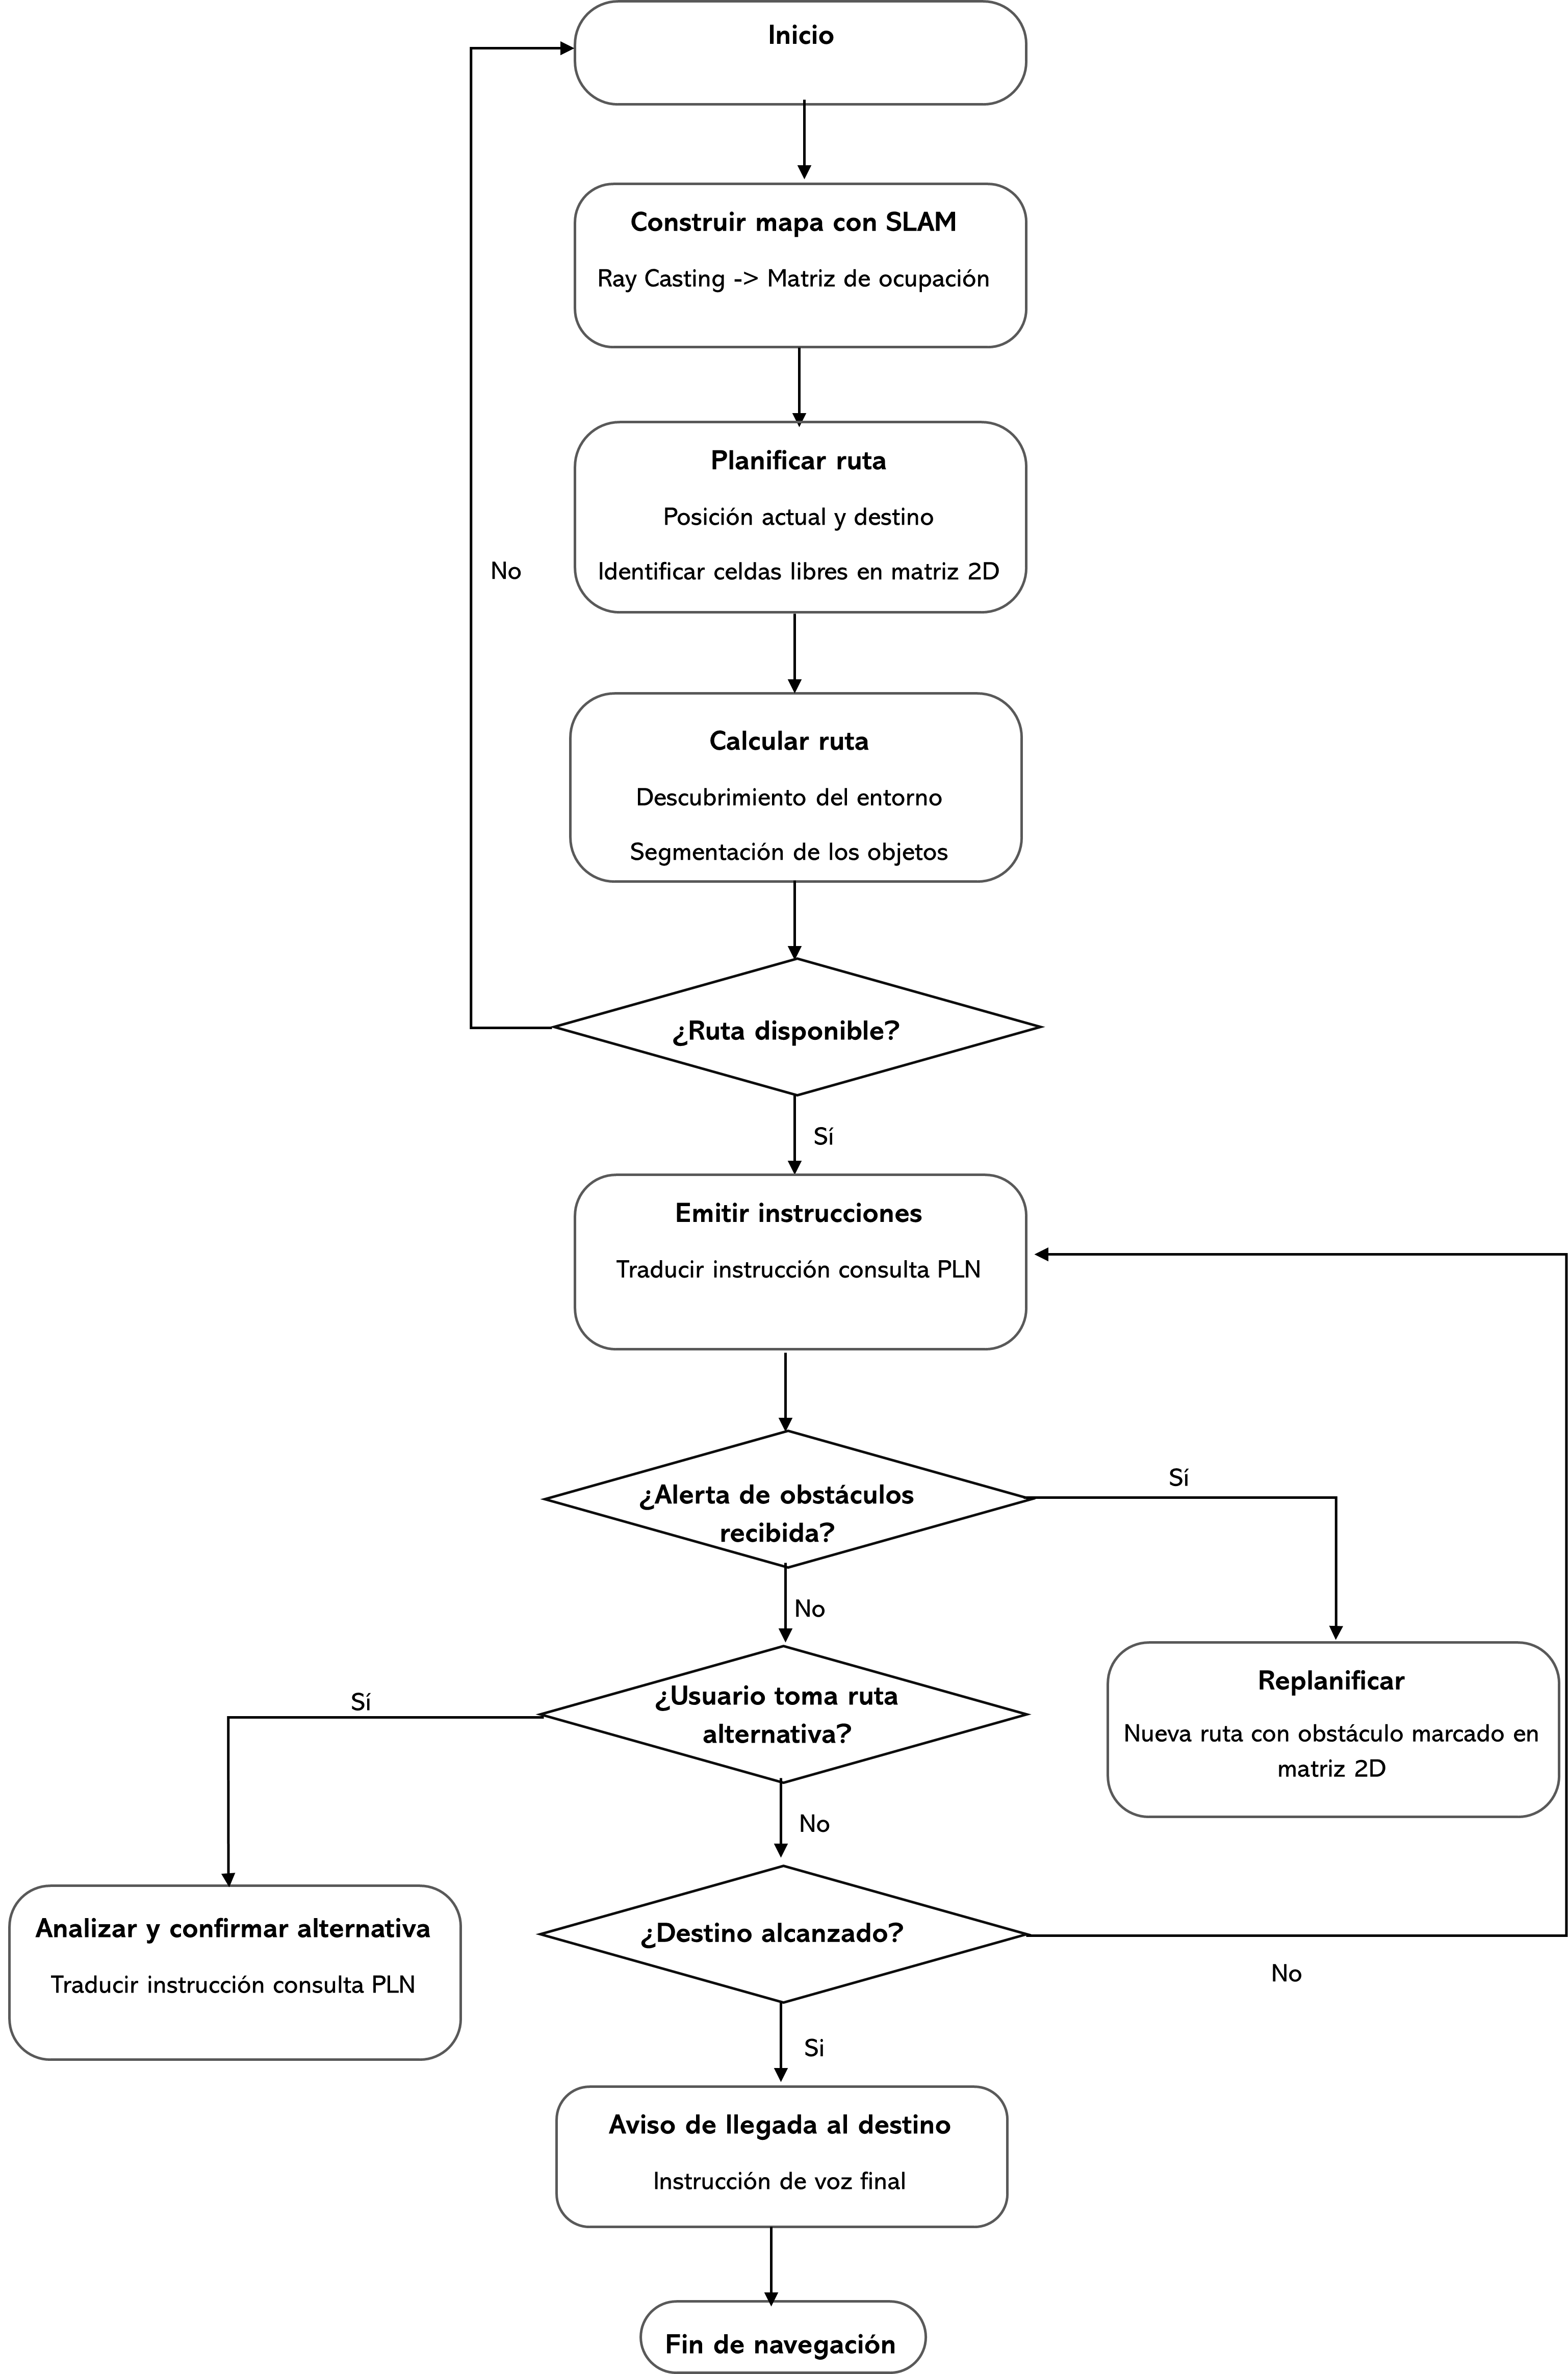
\includegraphics[width=11cm]{DiagFlujo/FlujoNavegacion.png}
    \caption{Diagrama de flujo del Modulo de Visión y Modulo sensorial}
    \label{fig:flujo_nav}
\end{figure}
El flujo inicia en el bloque Inicio y avanza hacia la construcción del entorno espacial mediante SLAM (Simultaneous Localization and Mapping), donde el sistema aplica Ray Casting para generar una matriz de ocupación 2D.

Con el mapa listo, el sistema ejecuta la planificación de ruta, identificando la posición actual, el destino y las celdas libres en la cuadrícula. 

A partir de esto, calcula la ruta mediante descubrimiento del entorno y segmentación de objetos. Si no existe una ruta disponible, el flujo regresa a planificar nuevamente. Cuando sí hay una ruta, se evalúa la condición ¿Ruta disponible? y el sistema procede a emitir instrucciones traducidas mediante procesamiento de lenguaje natural (PLN).

Desde ese punto se abre un ciclo de navegación activa:
Si llega una alerta de obstáculo, el sistema pasa a Replanificar, marcando el obstáculo en la matriz 2D y generando una nueva ruta, para luego volver a emitir instrucciones.

Si no hay alerta pero el usuario toma una ruta alternativa, el sistema la analiza y confirma mediante PLN.

Si no hay alerta y el usuario sigue la ruta, se evalúa si el destino fue alcanzado: si no, el ciclo regresa a emitir instrucciones; si sí, se emite un aviso de llegada por voz y el flujo concluye en Fin de navegación.

\subsection{Flujo de la Interacción}
Aquí se muestra como se comporta el flujo de los módulos de Reconocimiento de Voz, PLN y salida al usuario, permitiendo la interacción natural entre el usuario y el sistema de navegación asistida.

\begin{figure}[H]
    \centering
    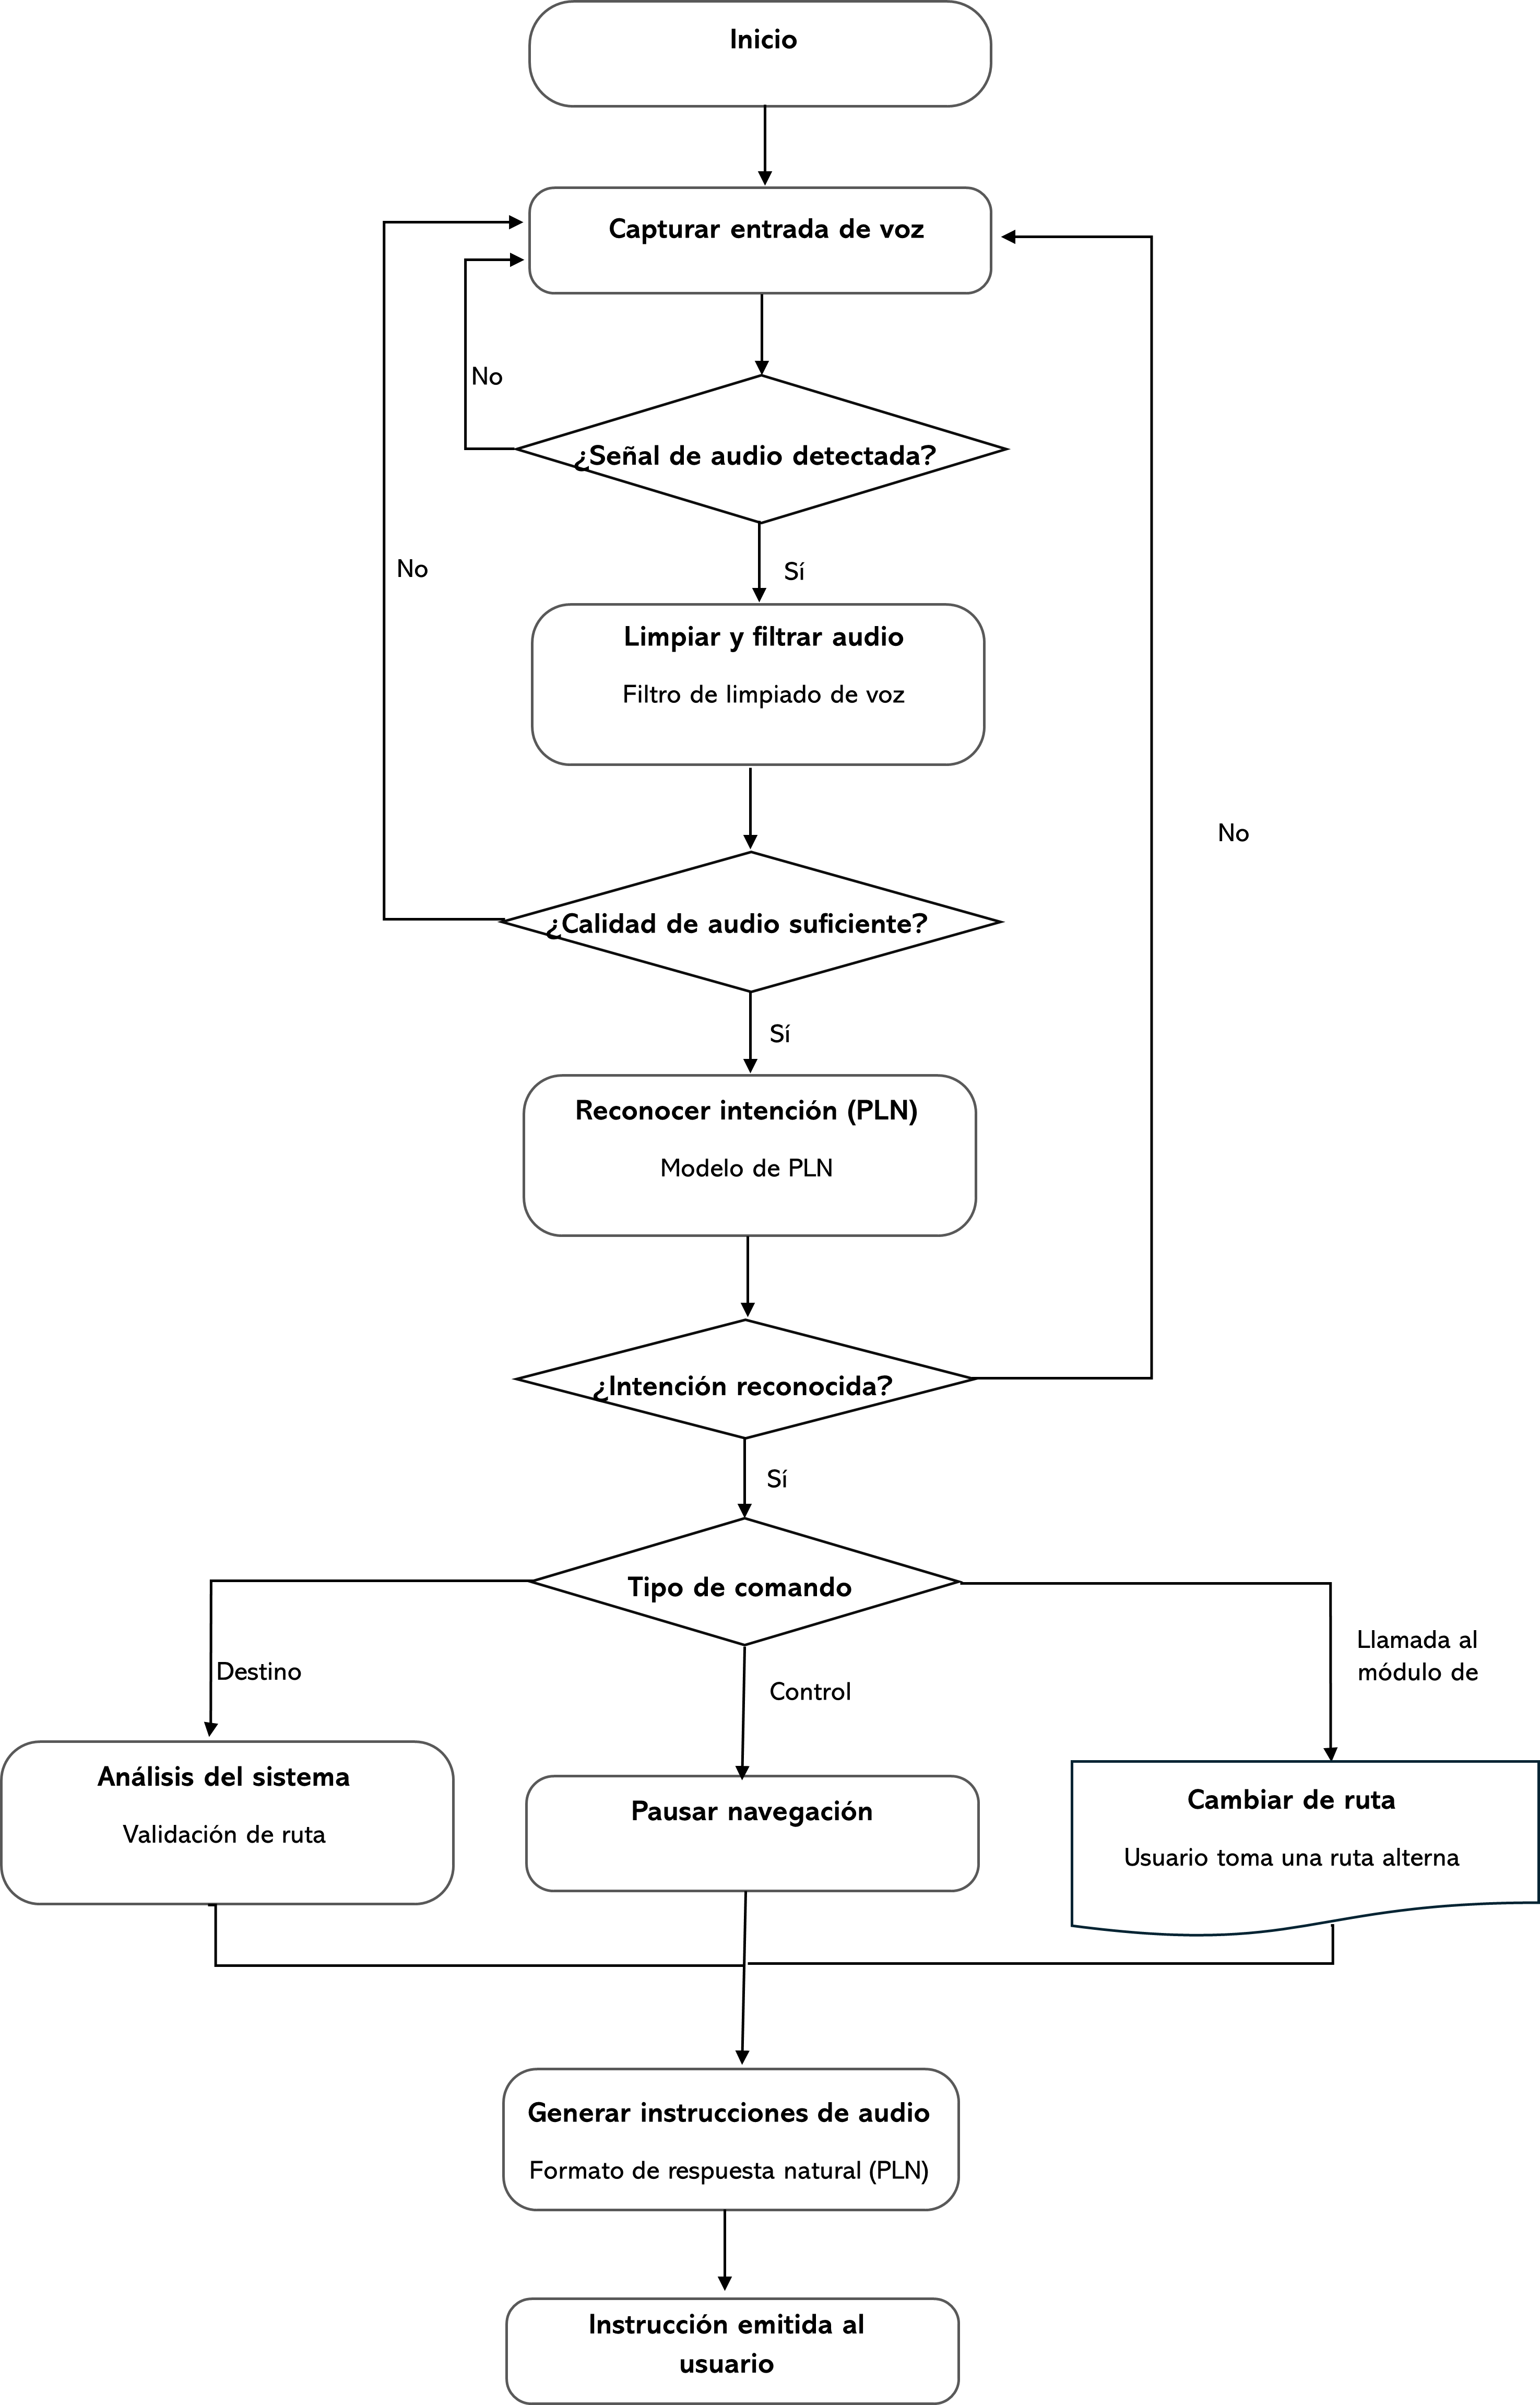
\includegraphics[width=11cm]{DiagFlujo/FlujoVozPLN.png}
    \caption{Diagrama de flujo del Modulo de Lenguaje Natural y Reconocimiento de voz}
    \label{fig:flujo_pln}
\end{figure}
El proceso inicia en el bloque “Inicio”, seguido de “Capturar entrada de voz”, donde el sistema activa el micrófono para adquirir señales de audio de manera continua.
Se evalúa la condición “¿Señal de audio detectada?”:
Si no se detecta señal, el sistema permanece en estado de espera y continúa monitoreando la entrada de audio.
Si se detecta señal, el flujo avanza al procesamiento de la misma.

Una vez detectada la señal, el sistema ejecuta el bloque “Limpiar y filtrar audio”, donde se aplican técnicas de reducción de ruido y mejora de calidad.
Se evalúa “¿Calidad de audio suficiente?”:
Si la calidad no es adecuada, el sistema descarta la señal y regresa a la captura, evitando interpretaciones erróneas.
Si la calidad es suficiente, el flujo continúa hacia el análisis semántico.
Este paso es fundamental para garantizar la confiabilidad del reconocimiento.

El sistema procesa la señal mediante el bloque “Reconocer intención (PLN)”, utilizando un modelo de procesamiento de lenguaje natural para interpretar el contenido del mensaje y se evalúa la condición “¿Intención reconocida?”:
Si no se reconoce la intención, el sistema vuelve al estado de captura, solicitando implícitamente una nueva entrada.
Si la intención es reconocida, el flujo continúa hacia la clasificación del comando.

Una vez comprendida la intención, el sistema clasifica la solicitud en el bloque “Tipo de comando”, distinguiendo tres puntos principales:
\begin{enumerate}
    \item Comandos de destino: Se dirigen al bloque “Análisis del sistema”, donde se realiza la validación de la ruta hacia el destino solicitado. Este proceso implica verificar la viabilidad del trayecto y preparar la navegación.
    \item Comandos de control: Incluyen acciones como “Pausar navegación”, permitiendo al usuario modificar el estado del sistema en tiempo real.
    \item Cambio de ruta: Corresponde al bloque “Cambiar de ruta”, donde el usuario solicita una alternativa. Este caso implica la comunicación con el módulo de navegación para recalcular el trayecto.
\end{enumerate}
Independientemente del tipo de comando, el sistema procede al bloque “Generar instrucciones de audio”, donde se construye una respuesta en lenguaje natural mediante técnicas de PLN.

Finalmente, se ejecuta “Instrucción emitida al usuario”, proporcionando retroalimentación auditiva clara y comprensible.

\section{Arquitectura}

A continuación se describe la arquitectura del sistema propuesto, la cual define los módulos que lo componen, su función dentro del flujo de procesamiento y la manera en que interactúan entre sí para lograr una navegación asistida coherente y en tiempo real.

\subsection{Diagrama de arquitectura}

El siguiente diagrama presenta la arquitectura modular del sistema de navegación asistida, mostrando cómo interactúan sus tres fuentes de entrada principales: la voz del usuario, la cámara y los sensores físicos. 

\begin{figure}[H]
    \centering
    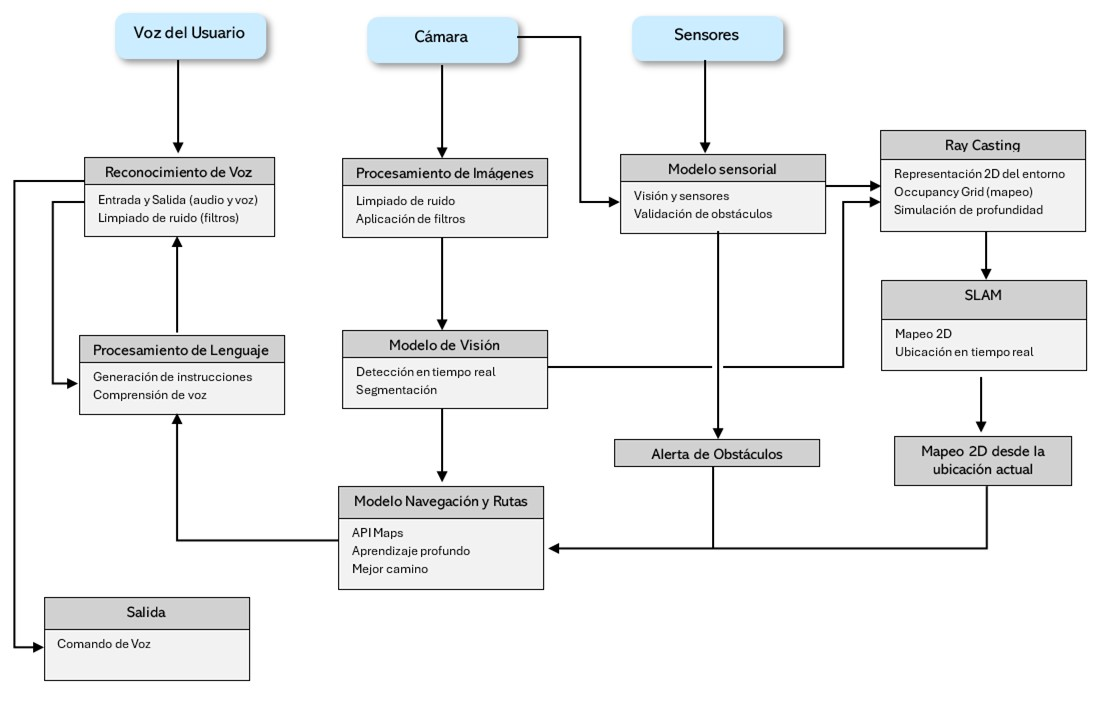
\includegraphics[width=17cm]{Diagramas/DiagArquitectura2.jpg}
    \caption{Diagrama de arquitectura general del sistema}
    \label{fig:arquitectura}
\end{figure}
El sistema tiene tres entradas principales: voz, cámara y sensores. La cámara pasa por procesamiento de imagen y luego por el modelo de visión, cuya tarea clave es la segmentación: detectar objetos y extraer sus coordenadas en el espacio (básicamente "hay un obstáculo en X, Y"). Esas coordenadas son una de las dos entradas más importantes al módulo de navegación.
\\
La entrada dada por el mapeo es resultante de la cadena generada por SLAM donde se obtiene un mapa en 2D con ubicación actual, el flujo se basa en los sensores y el Ray Casting que construye un Occupancy Grid, es decir, una rejilla que indica las celdas libres y ocupadas. Esa matriz 2D es literalmente el terreno sobre el que se calcula la ruta.
\\
El módulo de navegación y rutas recibe 3 entradas:
\begin{itemize}
    \item La matriz 2D con el mapa del entorno
    \item  Las coordenadas de objetos que detectó el modelo de visión (la segmentación)
    \item  Múltiples rutas basadas en la probabilidad de pesos que le asignan costo o preferencia a distintos caminos, así el sistema no solo busca el camino más corto geométricamente sino el más probable o seguro según la posibilidad de caminos que ha evaluado previamente el modelo.
\end{itemize}
Con esas tres entradas se calcula la mejor ruta.


Los sensores son alarmas en las que si detectan un obstáculo inesperado, generan una alerta que va directo al módulo de navegación para forzar un recalculado de la ruta, esto con el fin de evitar obstáculos. Esto es independiente del flujo normal, es una interrupción reactiva.
\\
La salida es dada con la ruta calculada, el sistema extrae las instrucciones paso a paso y las va entregando como salida de voz en tiempo real apoyado en la salida dada por el procesamiento de lenguaje que representa el sistema, también actualiza su estado interno conforme avanza, para dar las instrucciones adecuadas.

\section{Análisis de Requerimientos}

El presente capítulo tiene como objetivo establecer el puente entre los requerimientos
definidos en el capítulo anterior y las decisiones tecnológicas que dan forma a la
implementación del sistema. Cada tecnología elegida responde a uno o más requerimientos
concretos y se justifica con base en los fundamentos teóricos estudiados en el marco
teórico. El análisis se organiza por agrupación de módulos, siguiendo la misma
estructura arquitectónica del sistema.

Es importante señalar que la selección no se basa únicamente en la capacidad funcional
de cada tecnología, sino también en su viabilidad dentro de las restricciones
establecidas por los requerimientos no funcionales: operación en hardware embebido
de recursos limitados (RNF-05), operación autónoma sin conexión a internet (RNF-13)
y latencias de respuesta acotadas (RNF-01, RNF-02).

% ===
\subsection{Módulos de percepción}
% ======

Los módulos de percepción son el punto de entrada de toda la información que el sistema
procesa. Su función es transformar señales físicas ---fotogramas de cámara y lecturas
de sensores--- en representaciones computacionales útiles para los módulos posteriores.
Los requerimientos que gobiernan esta capa son especialmente exigentes en términos de
latencia (RNF-01), precisión (RNF-06) y eficiencia computacional (RNF-05), lo que
reduce significativamente el espacio de opciones tecnológicas viables.

\subsubsection{Preprocesamiento de imágenes: OpenCV y NumPy}

El requerimiento RF-07 establece que el sistema debe adquirir fotogramas de forma
continua y aplicar operaciones de preprocesamiento antes de alimentar el módulo de
visión. Según la literatura, el preprocesamiento transforma los datos visuales sin
procesar en un formato adecuado para el análisis posterior, eliminando distorsiones y
resaltando las características relevantes \cite{unitxlabs_prepost}. Operaciones como
redimensionamiento, normalización e igualación de contraste son necesarias porque un
modelo de detección produce resultados más estables cuando recibe entradas homogéneas,
reduciendo la variabilidad innecesaria debida a condiciones de iluminación o escala.

Para esta etapa se elige \textbf{OpenCV} (\texttt{cv2}) en combinación con
\textbf{NumPy}. OpenCV es una biblioteca de código abierto especializada en visión por
computadora que implementa de forma eficiente las operaciones de preprocesamiento
requeridas, y NumPy proporciona la estructura de datos matricial sobre la que se
representan las imágenes como arreglos numéricos. Ambas bibliotecas están ampliamente
documentadas, tienen una implementación madura y pueden ejecutarse sin aceleración GPU,
lo cual es indispensable dado que el hardware objetivo es una plataforma embebida
(RNF-05). Además, al operar localmente sin dependencia de servicios externos, se
garantiza el cumplimiento de RNF-13.

\subsubsection{Detección de objetos: YOLOv8}

El requerimiento central de los módulos de percepción es RF-08, que exige detectar
objetos relevantes para la navegación en cada fotograma con su localización espacial y
nivel de confianza. Este requerimiento se complementa con RF-09, que requiere asignar
a cada objeto una categoría semántica y un nivel de riesgo. Dado que el ciclo completo
desde la captura hasta la alerta no debe superar los 300~ms (RNF-01) y que la tasa de
detección correcta debe ser de al menos el 90\% (RNF-06), se necesita un modelo que
combine velocidad y precisión.

Como se estudió en el marco teórico, los detectores de una sola etapa como YOLO realizan
la extracción de características y la predicción de objetos en un único paso, lo que les
permite procesar imágenes con mayor velocidad que los detectores de dos etapas como
Faster R-CNN \cite{geeksforgeeks_object_detection}. YOLO divide la imagen en una
cuadrícula y predice simultáneamente las cajas delimitadoras y las clases presentes en
cada región \cite{geeksforgeeks_object_detection}, lo que lo convierte en la arquitectura
más adecuada para una aplicación con restricciones de latencia en tiempo real.

Se elige específicamente \textbf{YOLOv8} en su implementación de \textbf{Ultralytics},
ya que esta versión introduce mejoras arquitectónicas respecto a versiones anteriores,
mantiene compatibilidad con exportación en formato ONNX para optimización en plataformas
embebidas, y ofrece una API de uso directo en Python que simplifica la integración.
Además, su entrenamiento puede realizarse sobre conjuntos de datos especializados en
objetos relevantes para la navegación peatonal, lo que permite ajustar el modelo a los
casos de uso específicos del sistema (personas, puertas, escaleras, obstáculos estáticos).

\subsubsection{Detección de proximidad: sensores ultrasónicos}

El requerimiento RF-10 exige estimar la distancia entre el usuario y los objetos
detectados, y el requerimiento RF-11 establece que esta estimación debe validarse con
mediciones de sensores físicos para reducir falsas alarmas. La validación cruzada entre
visión y sensores tiene especial relevancia en situaciones donde la iluminación es baja
o cuando un objeto no se captura con suficiente claridad en la cámara.

Como se expone en el marco teórico, los sensores ultrasónicos miden distancias mediante
el tiempo de vuelo de un pulso sonoro y ofrecen una lectura sencilla y económica para
cortas y medias distancias \cite{hcsr04_datasheet}. Si bien los sensores ToF ofrecen
mayor precisión y menor tamaño \cite{vl53l1x_product}, los sensores ultrasónicos como
el HC-SR04 resultan suficientes para validar la presencia o ausencia de obstáculos
cercanos dentro de un rango de operación de 2~cm a 4~m \cite{hcsr04_datasheet}, que
cubre los casos críticos de navegación peatonal. Su implementación mediante el protocolo
I2C sobre la plataforma embebida es directa mediante bibliotecas como \texttt{smbus2}
o \texttt{RPi.GPIO}, sin requerir hardware adicional ni procesamiento significativo.

\subsubsection{Inferencia contextual y fusión sensorial}

El requerimiento RF-13 exige que el sistema infiera relaciones contextuales entre
objetos detectados, como el estado de apertura de una puerta o el grado de obstrucción
de un pasillo, para enriquecer la representación del entorno más allá de la detección
individual. El requerimiento RF-12 establece que el sistema solo debe emitir una alerta
al \emph{confirmar} un obstáculo, no al simplemente detectarlo, lo cual requiere un
mecanismo de validación probabilística.

Para esta función se adopta un modelo de \textbf{inferencia probabilística basada en
reglas}, implementado en Python. Este enfoque corresponde
al aprendizaje supervisado descrito en el marco teórico, donde la inferencia probabilística es la base para clasificación \cite{ibm2025_mltypes}. La elección de
un modelo probabilístico ligero, en lugar de una red neuronal compleja, responde
directamente a RNF-05: la inferencia contextual debe ejecutarse en hardware embebido
de recursos limitados sin introducir latencia adicional significativa al ciclo de
percepción. La fusión de la salida del módulo de visión con la lectura de sensores
se realiza mediante umbrales de confianza configurables, garantizando el comportamiento
conservador requerido por RNF-09.

% =====
\subsection{Módulos de representación}
% =======
Los módulos de representación transforman la información perceptual en una estructura
espacial que el módulo de navegación puede utilizar para planificar rutas. El mapa
generado debe distinguir zonas libres de zonas ocupadas (RF-16), actualizarse a una
frecuencia mínima de 10~Hz (RNF-03) y construirse de forma incremental sin necesidad
de un mapa previo (RF-15).

\subsubsection{Representación del entorno: occupancy grid con NumPy}

Como se estudió en el marco teórico, los mapas de ocupación representan el entorno
mediante una cuadrícula de celdas donde cada celda almacena la probabilidad de estar
ocupada por un obstáculo \cite{elfes1989}. Este concepto introducido por Elfes en 1989
es uno de los métodos más utilizados en robótica móvil para representar entornos
desconocidos, ya que cada celda puede clasificarse como libre, ocupada o desconocida
\cite{elfes1989}, lo cual corresponde exactamente a la representación requerida por
RF-16.

La \textit{occupancy grid} se implementa como una matriz bidimensional gestionada con
\textbf{NumPy}, aprovechando sus operaciones vectorizadas para actualizar múltiples
celdas en un solo paso. Esta elección garantiza eficiencia computacional (RNF-05) y
evita la necesidad de dependencias externas para el manejo matricial. La representación
en formato \textit{log-odds} permite actualizar probabilidades de ocupación de forma
incremental y numéricamente estable, acumulando observaciones a lo largo del tiempo.

\subsubsection{Estimación de posición: SLAM simplificado con EKF}

El requerimiento RF-14 exige mantener una estimación continua de la posición y
orientación del usuario integrando movimiento y percepción, y el requerimiento RF-15
añade que esta estimación debe construirse de forma incremental sin mapa previo. Estos
dos requerimientos describen conjuntamente el problema clásico de \textit{Simultaneous
Localization and Mapping} (SLAM), cuyo objetivo es estimar simultáneamente la pose del
agente y el mapa del entorno a partir únicamente de sus propias observaciones
\cite{wikipedia_slam}.

Dado que el hardware objetivo es una plataforma embebida con recursos limitados
(RNF-05), una implementación completa de SLAM como ORB-SLAM o LiDAR-SLAM sería
inviable: estos sistemas requieren procesamiento intensivo de nubes de puntos o de
descriptores visuales que excede la capacidad de una Raspberry Pi 4 operando en tiempo
real. Por ello se opta por un \textbf{SLAM simplificado orientado a mapeo local},
apoyado en un \textbf{Filtro de Kalman Extendido} (EKF) implementado en Python con
NumPy. Esta elección equilibra la necesidad de localización continua (RF-14) con la
restricción de recursos (RNF-05).

\paragraph{Representación del estado.}
La pose del usuario se modela como un vector de estado tridimensional:
\[
\mathbf{x}_t = [x_t,\; y_t,\; \theta_t]^T
\]
donde $(x_t, y_t)$ es la posición en el plano 2D y $\theta_t$ es la orientación.
Esta representación es suficiente para el dominio de navegación peatonal en superficies
planas y evita la complejidad computacional de una pose en 6 grados de libertad.

\paragraph{Modelo de movimiento (etapa de predicción).}
En cada ciclo, la pose se propaga hacia adelante usando los incrementos de odometría
$(\Delta d,\, \Delta\theta)$ estimados a partir del desplazamiento del usuario:
\[
\mathbf{x}_t^{-} = \mathbf{x}_{t-1} +
\begin{bmatrix}
\Delta d \cos(\theta_{t-1}) \\
\Delta d \sin(\theta_{t-1}) \\
\Delta\theta
\end{bmatrix}
\]
Este modelo de movimiento unicycle es no lineal en $\theta$, lo que justifica el uso
del EKF en lugar del filtro de Kalman estándar: el EKF linealiza localmente las
funciones no lineales mediante jacobianos, haciendo manejable la propagación de
incertidumbre sin abandonar el marco probabilístico \cite{thrun2005probabilistic}.
La covarianza del estado se propaga como:
\[
\mathbf{P}_t^{-} = \mathbf{F}\,\mathbf{P}_{t-1}\,\mathbf{F}^T + \mathbf{Q}
\]
donde $\mathbf{F}$ es el jacobiano del modelo de movimiento respecto al estado y
$\mathbf{Q}$ es la covarianza del ruido de proceso, que modela la incertidumbre
acumulada por la odometría aproximada.\cite{thrun2005probabilistic}.

\paragraph{Corrección con mediciones (etapa de actualización).}
Una vez obtenida la predicción, el EKF la corrige con las mediciones reales
provenientes de los sensores de proximidad. La ganancia de Kalman $\mathbf{K}$
determina cuánto peso se otorga a la medición frente a la predicción:
\[
\mathbf{K} = \mathbf{P}_t^{-}\mathbf{H}^T
             \bigl(\mathbf{H}\mathbf{P}_t^{-}\mathbf{H}^T + \mathbf{R}\bigr)^{-1}
\]
La pose y la covarianza se actualizan a partir de la innovación, es decir, la
diferencia entre la medición real $\mathbf{z}_t$ y la medición esperada
$h(\mathbf{x}_t^{-})$ según el modelo de observación $h(\cdot)$:
\[
\mathbf{x}_t = \mathbf{x}_t^{-} + \mathbf{K}\bigl(\mathbf{z}_t - h(\mathbf{x}_t^{-})\bigr)
\]
\[
\mathbf{P}_t = (\mathbf{I} - \mathbf{K}\mathbf{H})\,\mathbf{P}_t^{-}
\]
donde $\mathbf{H}$ es el jacobiano de $h(\cdot)$ respecto al estado y $\mathbf{R}$ es
la covarianza del ruido de medición de los sensores. Cuando la innovación es pequeña
(la predicción coincide bien con la medición) $\mathbf{K}$ se acerca a cero y se
confía más en el modelo; cuando es grande, $\mathbf{K}$ crece y la medición tiene
mayor peso sobre la estimación final. Este mecanismo autorregulado es lo que hace al
EKF robusto ante la acumulación de error de odometría \cite{thrun2005probabilistic}.

\paragraph{Actualización del mapa en log-odds.}
En paralelo a la estimación de la pose, el mapa de ocupación se actualiza de forma
incremental usando una representación en log-odds. Cada celda $c$ almacena el
logaritmo de la razón de probabilidades de estar ocupada frente a estar libre:
\[
l_t(c) = l_{t-1}(c) +
\log\frac{p(\mathbf{z}_t \mid c = \text{occ})}{p(\mathbf{z}_t \mid c = \text{free})}
\]
Esta representación tiene dos ventajas directas que justifican su elección. Primero,
la actualización es aditiva e incremental: cada nueva medición simplemente suma un
término al valor acumulado de la celda, sin necesidad de recalcular probabilidades
completas. Segundo, trabajar en escala logarítmica evita problemas numéricos de
underflow cuando las probabilidades se acercan a cero o a uno tras muchas
observaciones, lo que es frecuente en celdas cercanas al usuario
\cite{thrun2005probabilistic}. Los valores de log-odds se saturan en un rango
$[l_{\min},\, l_{\max}]$ para limitar el tiempo que el sistema tarda en corregir
una celda marcada erróneamente, garantizando que el mapa siga siendo actualizable
ante cambios dinámicos del entorno (RF-17).

\subsubsection{Actualización del mapa: ray casting con algoritmo de Bresenham}

El requerimiento RF-17 establece que el mapa debe actualizarse en respuesta a cambios
detectados en el entorno, y RNF-03 fija una frecuencia mínima de 10~Hz para esta
actualización. El mecanismo de actualización debe ser computacionalmente ligero para
no comprometer la latencia global del sistema.

Como se explica en el marco teórico, el ray casting permite proyectar rayos desde la
posición estimada del usuario para actualizar las celdas del mapa: las celdas recorridas
por el rayo se marcan como libres y la celda donde el rayo se detiene se marca como
ocupada \cite{elfes1989}. Para recorrer las celdas de forma eficiente se utiliza el
\textbf{algoritmo de Bresenham} \cite{bresenham1965}, que permite identificar las celdas
atravesadas por un rayo mediante operaciones aritméticas simples, sin multiplicaciones
ni divisiones en punto flotante. Como se señala en el marco teórico, el ray casting
presenta un bajo costo computacional, puede ejecutarse en CPU sin necesidad de GPU y es
compatible con mapas discretos basados en cuadrículas \cite{stackoverflow_raycasting},
lo que lo convierte en la técnica más adecuada para cumplir RNF-03 y RNF-05
simultáneamente, a diferencia del ray tracing, que requiere procesamiento
significativamente mayor \cite{stackoverflow_raycasting}.

% ====
\subsection{Módulo de navegación y rutas}
% ======

El módulo de navegación es el núcleo decisional del sistema. Debe calcular rutas
óptimas sobre el mapa local (RF-18), actualizarlas periódicamente (RF-19),
recalcularlas de forma inmediata ante obstáculos confirmados (RF-20), traducirlas
en instrucciones de movimiento (RF-21), resolver destinos sobre el mapa del entorno
(RF-22) y gestionar la seguridad del usuario como prioridad (RNF-09).

\subsubsection{Navegación local: aprendizaje por refuerzo profundo (DRL)}

A diferencia de los algoritmos clásicos de búsqueda de caminos como A* o Dijkstra,
que requieren un mapa completamente conocido y estático para operar de forma óptima
\cite{hart1968astar, dijkstra1959}, la navegación en entornos peatonales reales implica
incertidumbre, cambios dinámicos y necesidad de adaptación continua. El requerimiento
RF-19 establece que la ruta se recalcula periódicamente durante la navegación, pero
RF-20 exige recálculo inmediato ante un obstáculo confirmado: esta combinación describe
un agente que debe tomar decisiones secuenciales bajo incertidumbre, que es exactamente
el dominio del aprendizaje por refuerzo.

Como se estudió en el marco teórico, el aprendizaje por refuerzo es un enfoque en el
que un agente aprende a tomar decisiones mediante la interacción con su entorno,
recibiendo recompensas o penalizaciones, con el objetivo de aprender una política que
maximice la recompensa acumulada \cite{ibm2025_mltypes}. Al combinarlo con redes
neuronales profundas, el agente es capaz de aprender representaciones complejas del
entorno directamente desde los datos de los sensores, lo que lo hace especialmente
adecuado para espacios de estado continuos y entornos con obstáculos dinámicos como
los que enfrenta el sistema \cite{ibm2025_mltypes}.

Se propone el uso de \textbf{aprendizaje por refuerzo profundo} (DRL) para la
navegación local, con un espacio de acciones discreto compuesto por las cuatro
decisiones posibles del sistema: avanzar, girar a la izquierda, girar a la derecha
y detenerse. El estado del entorno se representa como un vector compacto que incluye
las distancias al obstáculo más cercano en cada dirección, la posición relativa al
siguiente waypoint y los niveles de riesgo detectados por el módulo de percepción.
La selección específica del algoritmo de entrenamiento, el entorno de simulación y
la estrategia de transferencia al hardware real se definirán en la segunda etapa del
trabajo terminal, una vez validado el comportamiento del resto de los módulos del
sistema.

\subsubsection{Submódulo de dirección: traducción de acciones}

El requerimiento RF-21 exige que la acción elegida por el modelo se traduzca en una
instrucción discreta y comprensible para el usuario. Dado que el espacio de acciones
del modelo de RL es ya discreto (avanzar, girar izquierda, girar derecha, detenerse),
esta traducción puede implementarse mediante \textbf{reglas determinísticas simples}
en Python: cada índice de acción se mapea directamente a una instrucción de texto con
distancia y ángulo aproximados. La complejidad del sistema se concentra en el modelo de
decisión; la capa de traducción no requiere aprendizaje ni módulos adicionales. Esto
garantiza latencia baja y comportamiento predecible, alineándose con RNF-09.

\subsubsection{Módulo de alerta de obstáculos: capa de seguridad por umbrales}

El requerimiento RF-12 establece que al confirmar un obstáculo el sistema debe notificar
al usuario de forma inmediata y desencadenar el recálculo de ruta. El requerimiento
RNF-09 añade que ante baja confianza el sistema debe optar por la acción más
conservadora. Estos requerimientos describen una capa de seguridad independiente del
modelo de RL, que actúa como interruptor prioritario.

Esta capa se implementa mediante \textbf{umbrales determinísticos} sobre la distancia
estimada y el nivel de riesgo asignado por el módulo de percepción. Si la distancia al
obstáculo confirmado cae por debajo de un umbral de alerta, el sistema emite la alerta
por voz y notifica al módulo de navegación para recalcular, independientemente de la
decisión del modelo de RL. Este diseño garantiza el comportamiento conservador exigido
por RNF-09 sin depender del umbral de confianza del modelo, que podría variar en
entornos poco estructurados.

\subsubsection{Resolución de destinos sobre el mapa del entorno}

El requerimiento RF-22 establece que el usuario debe poder indicar como destino un
elemento del entorno, como una puerta o la salida. En el diseño original se consideró
un servicio de cartografía digital con GPS para rutas a nivel de ciudad; sin embargo,
este enfoque depende de conexión a internet, tiene una precisión de varios metros y no
funciona en interiores, que es precisamente donde el sistema resulta más útil. Por
ello se decidió resolver los destinos sobre el propio mapa que construye el sistema:
el módulo SLAM conserva la etiqueta semántica de cada objeto reconocido, de modo que
una petición como ``llévame a la salida'' se traduce en la posición de la puerta
registrada más cercana, y la navegación local guía al usuario hacia ella. Esta
solución opera sin internet, en concordancia con RNF-13.

% ======
\subsection{Módulos de interacción}
% =========

Los módulos de interacción son la interfaz entre el sistema y el usuario. Dado que
el sistema está orientado a personas con discapacidad visual, toda la interacción
debe realizarse exclusivamente por voz (RF-06, RNF-10), sin requerir interfaz visual
en ningún momento. Los requerimientos imponen restricciones de latencia de 500~ms para
el reconocimiento de comandos (RNF-02) y una tasa de reconocimiento correcto de al
menos el 92\% en entornos con hasta 60~dB de ruido ambiental (RNF-07). Dado que
el sistema debe operar sin conexión a internet (RNF-13), todos los componentes de
interacción deben funcionar de forma local.

\subsubsection{Captura y preprocesamiento de audio: PyAudio}

El requerimiento RF-01 establece que el sistema debe capturar audio de forma continua
y detectar automáticamente segmentos de voz activa. El requerimiento RF-02 añade que
debe aplicarse supresión de ruido antes de entregar la señal al módulo de
reconocimiento.

Se utiliza \textbf{PyAudio} como interfaz de captura de audio, ya que proporciona
acceso de bajo nivel al micrófono del dispositivo en Python y es compatible con la
plataforma embebida objetivo. La detección de actividad de voz (VAD) se implementa
mediante un umbral de energía sobre el nivel de la señal capturada, descartando
segmentos de silencio para reducir el volumen de datos enviados al módulo de
reconocimiento. El preprocesamiento de reducción de ruido se aplica mediante filtros
sobre el flujo de audio antes de pasarlo al reconocedor, cumpliendo RF-02 sin
introducir dependencias de servicios en la nube.

\subsubsection{Reconocimiento de voz: Vosk}

El requerimiento RF-03 exige transcribir la señal de voz a texto e interpretar la
intención del usuario. Las restricciones RNF-13 (sin internet) y RNF-02 (latencia
$<$ 500~ms) descartan motores de reconocimiento basados en la nube como Google Speech
o Whisper en su versión en línea, ya que dependen de conectividad e introducen latencia
de red variable.

Se elige \textbf{Vosk} como motor de reconocimiento automático de voz (ASR) porque
opera completamente de forma local (\textit{offline}), ofrece modelos en español de
tamaño reducido compatibles con hardware embebido de recursos limitados, y su API en
Python permite integrar reconocimiento continuo en tiempo real con baja latencia. Vosk
cumple directamente RNF-13 al no requerir internet, y su ejecución local garantiza una
latencia de reconocimiento dentro de los 500~ms establecidos por RNF-02 en condiciones
normales de operación.

\subsubsection{Procesamiento de lenguaje natural: spaCy y clasificación por reglas}

Una vez transcrito el texto, el sistema debe interpretar la intención del usuario (RF-03) y reconocer comandos para controlar la sesión como pausar, reanudar o detener la navegación (RF-05). Los comandos del sistema son un conjunto cerrado y predecible de intenciones (indicar destino, solicitar descripción, controlar sesión), lo que permite implementar un clasificador de intenciones sin necesidad de un modelo de lenguaje grande.

Una vez transcrito el texto, el sistema debe interpretar la intención del usuario (RF-03) y reconocer comandos para controlar la sesión como pausar, reanudar o detener la navegación (RF-05). Los comandos del sistema son un conjunto cerrado y predecible de intenciones (indicar destino, solicitar descripción, controlar sesión), lo que permite implementar un clasificador de intenciones sin necesidad de un modelo de lenguaje grande.
El texto transcrito se normaliza previamente mediante tokenización y lematización con spaCy, eliminando palabras vacías para reducir el espacio de representación. 
Se emplea \textbf{spaCy} para el análisis morfológico y la extracción de entidades del texto transcrito, combinado con un clasificador de intenciones basado en reglas y similitud de patrones implementado en Python. 
Este enfoque opera localmente sin internet (RNF-13) y su ejecución es prácticamente instantánea, lo que contribuye a mantener la latencia global dentro de RNF-02. Si la complejidad de los comandos crece en iteraciones futuras del sistema, la modularidad de esta capa (RNF-14) permite sustituir el clasificador SVM por un modelo más sofisticado sin afectar el resto del sistema.

Para la etapa de clasificación de intenciones se considera como esquema de vectorización. Esta representación pondera cada término en función de su frecuencia en el comando y su rareza relativa en el corpus de entrenamiento, de modo que las palabras clave con mayor poder discriminativo, como los verbos de acción o los nombres de destino, reciben mayor peso que términos genéricos. Dado que el conjunto de intenciones del sistema es cerrado y el vocabulario de comandos es acotado y predecible, TF-IDF captura la señal suficiente para separar las clases de forma efectiva sin incurrir en el costo computacional de representaciones más complejas.

\subsubsection{Síntesis de voz: pyttsx3}

El requerimiento RF-04 establece que el sistema debe convertir en audio las
instrucciones de navegación, alertas y respuestas, reproduciéndolas mediante síntesis
de voz con lenguaje natural y frases cortas. El requerimiento RNF-11 añade que las
instrucciones deben ser claras y usar referencias espaciales concretas, y RNF-12 exige
que la retroalimentación se emita de forma proactiva ante eventos relevantes sin esperar
solicitud del usuario.

Se elige \textbf{pyttsx3} como motor de \textit{Text-to-Speech} (TTS) porque opera
completamente de forma local sin depender de servicios en línea (RNF-13), es compatible
con la plataforma embebida objetivo mediante ALSA/PulseAudio, y permite ajustar la
velocidad de habla y el volumen para mejorar la comprensibilidad de las instrucciones
(RNF-11). Su integración en Python es directa y añade una latencia de síntesis baja
para textos cortos, lo que permite la retroalimentación proactiva requerida por RNF-12
ante eventos como detección de obstáculos o cambios de ruta.

\section{Selección y justificación de hardware principal}

\subsection{Comparación de sensores de distancia para dispositivos portables}

La selección del sensor de distancia representa un aspecto crítico en el diseño de sistemas de navegación asistida. En dispositivos portables como gafas inteligentes, los sensores deben cumplir con requisitos estrictos de tamaño reducido, bajo consumo energético y suficiente alcance para detectar obstáculos con anticipación.

Existen diversos tipos de sensores que pueden emplearse para este propósito, entre los que destacan sensores ultrasónicos básicos, sensores ultrasónicos industriales de alta precisión, sensores Time-of-Flight (ToF) y sensores LiDAR compactos. Cada tecnología presenta ventajas y limitaciones que deben considerarse en función del entorno de operación y las restricciones del dispositivo.

La Tabla~\ref{tabla_sensores_completa} muestra una comparación entre algunos sensores comerciales ampliamente utilizados en sistemas embebidos y robótica.

\begin{table}[H]
\centering
\begin{tabular}{llllll}
\hline
Sensor & Tipo & Alcance & Precisión & Tamaño & Interfaz \\
\hline
HC-SR04 \cite{hcsr04_datasheet}          & Ultrasónico & 2~cm -- 4~m    & $\pm3 mm$    & $45x20x15 mm$      & Trigger/Echo \\
MB1232 \cite{mb1232_datasheet}           & Ultrasónico & 20~cm -- 7.65~m & $\pm1 mm$     & $14.4x15.5x15.5mm$ & I2C \\
VL53L0X \cite{vl53l0x_datasheet}         & ToF         & hasta 2~m      & $\pm3\%$     & $4.4x2.4x1.0 mm$ & I2C \\
VL53L1X \cite{vl53l1x_datasheet}         & ToF         & hasta 4~m      & $\pm20 mm$     & $4.9x2.5x1.5 mm$ & I2C \\
TF-Mini  \cite{tfmini_datasheet}          & LiDAR       & hasta 12~m     & $\pm6 cm$ & $42x15x16 mm$    & UART/I2C \\
Lidar Lite v3 \cite{lidarliitev3_manual}  & LiDAR       & hasta 40~m     & $\pm25 cm$ & $40x48x20 mm $      & I2C/PWM \\
\hline
\end{tabular}
\caption{Comparación de sensores de distancia utilizados en sistemas embebidos \cite{hcsr04_datasheet, mb1232_datasheet, vl53l0x_datasheet, vl53l1x_datasheet, tfmini_datasheet, lidarliitev3_manual}.}
\label{tabla_sensores_completa}
\end{table}

Como puede observarse, los sensores ultrasónicos básicos como el HC-SR04 \cite{hcsr04_datasheet} presentan un costo bajo pero su tamaño físico y precisión limitada los hacen menos adecuados para dispositivos portables en entornos ruidosos. El sensor MB1232 \cite{mb1232_datasheet} resuelve estas limitaciones manteniendo el principio ultrasónico: ofrece un alcance de hasta 7.65~m, resolución de 1~cm, interfaz I2C, calibración automática en tiempo real y un tamaño inferior a una pulgada cúbica, lo que lo convierte en la opción más adecuada para el presente trabajo terminal.

En contraste, sensores ToF como el VL53L1X \cite{vl53l1x_datasheet} ofrecen alta precisión pero a alcances más limitados (hasta 4~m), y los sensores LiDAR compactos como el TF-Mini \cite{tfmini_datasheet} proporcionan mayor alcance pero con un consumo energético y costo superiores.

En el contexto del sistema de gafas inteligentes para navegación asistida desarrollado en este trabajo, el MB1232 representa la solución idónea, ya que combina el mayor alcance de la categoría ultrasónica compacta, alta tolerancia al ruido acústico y eléctrico de entornos urbanos, bajo consumo energético y la interfaz I2C requerida para su integración con la plataforma Raspberry Pi \cite{mb1232_datasheet}.

\subsection{Comparación de módulos de cámara para sistemas embebidos}

Las cámaras utilizadas en sistemas de visión por computadora deben proporcionar imágenes con suficiente resolución y calidad para permitir la detección y reconocimiento de objetos mediante algoritmos de inteligencia artificial.

En dispositivos portables, los módulos de cámara deben además cumplir con restricciones de tamaño y consumo energético \cite{raspberrypi_camera_doc3}.

La Tabla~\ref{tabla_camaras} presenta una comparación entre algunos módulos de cámara ampliamente utilizados en plataformas embebidas.

\begin{table}[H]
\centering
\begin{tabular}{llllll}
\hline
Modelo & Sensor & Resolución & Tamaño & Interfaz & Uso común \\
\hline
OV2640 \cite{ov2640_datasheet}              & OmniVision & 2 MP  & $21 \times 12.5mm$ & SPI/DVP  & IoT, ESP32-CAM \\
OV5647 \cite{raspberrypi_camera_doc}        & OmniVision & 5 MP  & $25 \times 24mm$     & CSI      & Raspberry Pi \\
IMX219 \cite{arducam_imx219}               & Sony       & 8 MP  & $25 \times 24mm$     & CSI      & Raspberry Pi v2 \\
IMX477 \cite{raspberrypi_camera_doc}        & Sony       & 12 MP & $38 \times 38mm$       & CSI      & Visión avanzada \\
IMX708 \cite{raspberrypi_camera_doc3} & Sony & 12 MP & $25 \times 24mm$ & MIPI CSI-2 & Raspberry Pi v3 \\
ArducamMini \cite{arducam_imx219}          & Variado    & 2--12 MP & $21 \times 12.5mm$ & SPI/I2C & Sistemas embebidos \\
\hline
\end{tabular}
\caption{Comparación de módulos de cámara para aplicaciones embebidas \cite{ov2640_datasheet, raspberrypi_camera_doc, raspberrypi_camera_doc3,arducam_imx219}.}
\label{tabla_camaras}
\end{table}

Entre los módulos presentados, el Raspberry Pi Camera Module 3 con sensor IMX708 \cite{raspberrypi_camera_doc3} destaca como la opción más adecuada para el presente trabajo terminal. Su sensor Sony de 12~MP con tecnología back-illuminated stacked CMOS ofrece imágenes de alta resolución y calidad incluso en condiciones de baja iluminación, mientras que el sistema de autoenfoque por detección de fase (PDAF) garantiza nitidez sobre objetos a distintas distancias sin intervención manual. El modo HDR resulta especialmente valioso para mantener la calidad de imagen en entornos urbanos con variaciones abruptas de iluminación, como transiciones entre interiores y exteriores. Adicionalmente, su compatibilidad nativa con Raspberry Pi y soporte completo por parte de la biblioteca \texttt{libcamera} simplifican considerablemente el desarrollo del sistema de visión por computadora basado en inteligencia artificial propuesto en este trabajo \cite{raspberrypi_camera_doc3}.

% ======
\subsection{Resumen de decisiones tecnológicas}
% ====

La Tabla~\ref{tabla_tecnologias} resume las tecnologías seleccionadas para cada módulo
del sistema, los requerimientos que motivan cada elección y los fundamentos teóricos
que la respaldan.

\begin{table}[H]
\centering
\renewcommand{\arraystretch}{1.3}
\begin{tabular}{p{3.2cm} p{3.5cm} p{3.2cm} p{3.2cm}}
\hline
\textbf{Módulo} & \textbf{Tecnología} & \textbf{Requerimientos} & \textbf{Fundamento teórico} \\
\hline
Preprocesamiento & OpenCV + NumPy & RF-07, RNF-05, RNF-13 & \cite{unitxlabs_prepost} \\
Detección de objetos & YOLOv8 (Ultralytics) & RF-08, RF-09, RNF-01, RNF-06 & \cite{geeksforgeeks_object_detection} \\
Proximidad sensorial & Sensores ultrasónicos + smbus2 & RF-10, RF-11 & \cite{hcsr04_datasheet} \\
Fusión e inferencia & Clasificación por reglas probabilísticas en Python & RF-11, RF-12, RF-13, RNF-09 & \cite{ibm2025_mltypes} \\
\hline
Mapa de ocupación & Occupancy grid + NumPy & RF-15, RF-16, RNF-03, RNF-05 & \cite{elfes1989} \\
Localización & SLAM simplificado + EKF & RF-14, RF-15, RNF-05 & \cite{thrun2005probabilistic} \\
Actualización del mapa & Ray casting (Bresenham) & RF-17, RNF-03 & \cite{elfes1989, bresenham1965} \\
\hline
Navegación local & RL con PPO (SB3 + PyTorch) & RF-18, RF-19, RF-20, RNF-04 & \cite{ibm2025_mltypes} \\
Alerta de obstáculos & Umbrales determinísticos & RF-12, RF-20, RNF-09 & --- \\
Instrucciones & Reglas de dirección en Python & RF-21, RNF-11 & --- \\
Resolución de destinos & \emph{Landmarks} etiquetados del SLAM & RF-22, RF-23, RNF-13 & \cite{thrun2005probabilistic} \\
\hline
Captura de audio & PyAudio + VAD & RF-01, RF-02, RNF-02 & --- \\
Reconocimiento de voz & Vosk (offline ASR) & RF-03, RF-05, RNF-07, RNF-13 & --- \\
PLN e intención & spaCy + reglas & RF-03, RF-05, RNF-02 & --- \\
Síntesis de voz & pyttsx3 (offline TTS) & RF-04, RNF-11, RNF-12, RNF-13 & --- \\
\hline
\end{tabular}
\caption{Resumen de tecnologías seleccionadas por módulo con sus requerimientos asociados.}
\label{tabla_tecnologias}
\end{table}